\section{Добијање одговора на задати упит}

\subsection{Одговори на упите}

Претраживач би имао мало или нимало смисла ако корисник не би могао да уноси кључне речи за претраживање и да на основу њих добије одговарајуће хипервезе. Зато је поред хипервеза потребно имати и кључне речи које се помињу на тим странама.

Према раније описаној схеми веб претраживања, потребно је да се направи листа (или мапа, што ће бити описано у каснијем току овог рада) \textbf{index}, која би се састојала од листи, које би опет имале једно поље за кључну реч и остала поља за хипервезе где се помиње та реч.

Дакле, прво се креира листа која садржи листу. Кључна реч ће бити у нултом пољу те листе, а у осталим ће постојати хипервезе везане за ту кључну реч (види слику \ref{slike:indeks1}).

\begin{figure}[here]
\centering
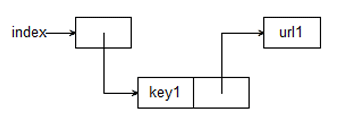
\includegraphics[height=75px, width=200px]{index1.png}
\caption{Креирање првог поља у индексу}
\label{slike:indeks1}
\end{figure}

После иницијалног дела могуће је даље додавати нове листе у индекс, где је почетно поље такође кључна реч (слика \ref{slike:index2}).\\

\begin{figure}[here]
\centering
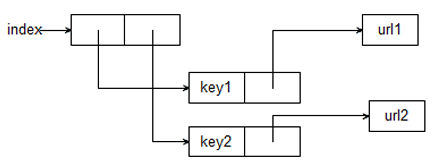
\includegraphics[height=100px, width=260px]{index2.png}
\caption{Следећа кључна реч и њена хипервеза}
\label{slike:index2}
\end{figure}

Међутим, могуће је да постоји више хипервеза који су везани за исту кључну реч. У том случају, додаје се ново поље листи у којој је та кључна реч (слика \ref{slike:index3}).

\begin{figure}[here]
\centering
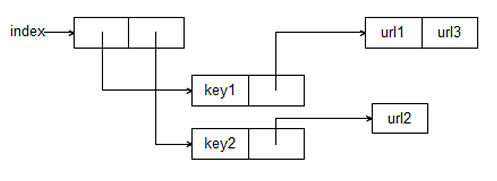
\includegraphics[height=110px, width=300px]{index3.png}
\caption{Два хиперлинка са истом кључном речју}
\label{slike:index3}
\end{figure}

За прављење и коришћење индекса, потребне су три процедуре:

\begin{description}
\item[add to index] - процедура која додаје кључну реч и хипервезу у индекс;
\item[lookup] - враћа листу свих хипервеза на основу кључне речи;
\item[add page to index] - садржај странице (HTML к\^{о}д) раставља на кључне речи и убацује их у индекс.
\end{description}

У наредним поглављима биће размотрени к\^{о}дови поменутих процедура.

\subsubsection{Прављење индексa}

Процедура додавања кључних речи и хипервеза у индекс, узима три податка: index (листа) и две ниске - кључну реч (keyword) и хипервезу(url).

\begin{lstlisting}[caption=Процедура add\_to\_index, label={lst:addtoindex}, numbers=left]
def add_to_index(index, keyword, url):
    for entry in index:
        if entry[0]==keyword:
            entry[1].append(url)
            return  # ne vraca se nista, samo se menja index
    index.append([keyword, [url]])
\end{lstlisting}

Ова процедура прелистава индекс и ако наиђе кључна реч која постоји у индексу, онда само додаје нову хипервезу у листу хипервеза, а ако кључна реч не постоји у индексу, додаје нову листу у индекс, са једном хипервезом.

\subsubsection{Процедура за претраживање индекса}

Процедура тражења узима два податка: index (листа) и кључну реч (ниска).

\begin{lstlisting}[caption=Процедура lookup, label={lst:lookup}, numbers=left]
def lookup(index, keyword):
    lookup_list = []
    for entry in index:
        if entry[0]==keyword:
            for entry_url in entry[1]:
                lookup_list.append(entry_url)
    return lookup_list
		\end{lstlisting}

Процедура прво прави привремену листу и претражује индекс, тражећи кључну реч. Када је нађе, онда сваку хипервезу везану за ту кључну реч, поставља у привремену листу и њу враћа као резултат.

% \pagebreak

\subsubsection{Градња индекс листе}

Сад кад је позната процедурa add\_to\_index, могуће је дати к\^{о}д процедуре\\ add\_page\_to\_index, која има три аргумента: индекс листу, хипервезу као ниску и садржај странице такође као ниску. Ова процедура служи за прављење индекса.

\begin{lstlisting}[caption=Процедура add\_page\_to\_index , label={lst:addpagetoindex}, numbers=left]
def add_page_to_index(index, url, content):
    for entry in content.split():
        add_to_index(index, entry, url)
		\end{lstlisting}

Процедура читав садржај странице раставља на речи (празан карактер је подразумевана вредност за сепаратор) и онда се сваку реч додаје у индекс заједно са хипервезом.

\subsubsection{Промена веб-паука да ради са индексом}
Пошто су наведене ове три кључне процедуре к\^{о}д измењеног веб-паука тако да ради са индексом.

\begin{lstlisting}[caption=Веб-паук који ради са индексом, label={lst:crawler}, numbers=left]
def get_page(url):
    try:
        import urllib
        return urllib.urlopen(url).read()
    except:
        return ""
def union(a, b):
    for e in b:
        if e not in a:
             a.append(e)
def get_next_target(page):
    start_link = page.find('<a href=')
    if start_link == -1:
        return None, 0
    start_quote = page.find('"', start_link)
    end_quote = page.find('"', start_quote + 1)
    url = page[star_quote + 1: end_quote]
    return url, end_quote
def get_all_pages(page):
    while True:
        links = []
        url, endpos = get_next_target(page)
        if url:
            links.append(url)
            page = page[endpos:]
        else:
            break
    return links

# kreiranje indexa

def add_to_index(index, keyword, url):
    for entry in index:
        if entry[0] == keyword:
            entry[1].append(url)
            return
    index.append([keyword, [url]])
def add_page_index(index, url, content):
    for entry in content.split():
        add_to_index(index, entry, url)

# glavna funkcija

def crawl_web(seed):
    tocrawl = [seed]
    crawled = []
    index = [] # inicijalizacija indexa
    while tocrawl:
        page = tocrawl.pop()
        if page not in crawled:
            content = get_page(page)
            add_page_to_index(index, page, content)
            union(tocrawl, get_all_pages(content))
            crawled.append(page)
    return crawled
\end{lstlisting}

Ако се овом  к\^{о}ду придода и к\^{о}д процедуре \emph{lookup}, онда се добијају резултати у облику листе свих хипервеза које одговарају траженој кључној речи. Следи дата процедура која ради са индексом:

\begin{lstlisting}[caption=Процедура lookup која ради са индексом, label={lst:lookup_index}, numbers=left]
def lookup(index,keyword):
    lookup_list = []
    for entry in index:
        if entry[0]==keyword:
            for entry_url in entry[1]:
                lookup_list.append(entry_url)
    return lookup_list
\end{lstlisting}

Већ сад је могуће добити све хипервезе у односу на тражену кључну реч. За резултате погледати поглавље \ref{sec:dodatakb}.
%\pagebreak
\subsection{Како убрзати?}

У претходним поглављима овог рада је изграђен систем који може да одговори на упите, тако што ће проверити једну кључну реч из индекса у једном тренутку. Претраживач ће преко \textbf{lookup} процедуре проверити да ли у индексу постоји кључна реч која је постављена у упит и онда на основу тога дати одговарајући резултат.

Ипак, са великим индексом и већим бројем упита, овакав систем ће се испоставити као \emph{спор}. Типични претраживач би требало да одговори на упите за мање од секунде, ако не и много брже. Закључак је да претраживач мора да ради брже са великим индексом.

Поставља се питање шта је потребно да би неки програм боље радио, одн. узимао што мање ресурса, а у исто време што брже достављао тражене резултате. Наравно, при томе не сме да се доведе у питање тачност и квалитет рада. Када програми постану велики, потребно је водити рачуна о томе колико ,,коштају'' када их покренемо. Евалуација трошкова једног програма приликом његовог рада, је веома важна и представља један од највећих проблема у рачунарству. Поступак евалуације се назива \emph{анализа алгоритма}\index{algoritam@алгоритам!analiza algoritma@анализа алгоритма}\footnote{Под алгоритмом подразумевамо било коју добро дефинисану процедуру која узима неку вредност или скуп вредности као \emph{улаз} и као резултат даје неку вредност или скуп вредности као \emph{излаз}.\cite{cormen2001introduction}}

Цена алгоритма зависи од улаза. Цена се касније испоставља у већој потрошњи ресурса рачунара. Претпоставимо да имамо два различита алгоритма Алго1 и Алго2, који успешно решавају исти проблем:

\begin{itemize}
\item Улаз $\longrightarrow$ Алго1 $\longrightarrow$ Резултат
\item Улаз $\longrightarrow$ Алго2 $\longrightarrow$ Резултат
\end{itemize}

Није могуће поставити фиксну цену и рећи конкретну суму колико коштају сваки од ова два алгоритма. За неке улазе, Алго1 ће бити јефтинији него Алго2, али за друге улазе, ситуација ће бити другачија. Другим речима, потребно је предвидети цену, а да се не анализира алгоритам за сваки улаз.

Количина улазних података је главни фактор који утиче на брзину алгоритма, одн. цена извршења програма је директно пропорционална односа између повећања улазних података и повећања времена које је потребно да се изврши програм.

Дакле, потребно је знати која је цена (време, меморија) извршења једног програма у зависности од количине улазних података. Такође, потребно је посебно анализирати најгору могућу ситуацију приликом процеса претраживања. Са  \textbf{lookup} процедуром и индексом чији к\^{о}д је наведен у претходном поглављу, најгори случај би био ако се кључна реч која се тражи у упиту налази на крају индекс листе. Тако да, независно од количине улазних података (индекс), не може се са сигурношћу предвидедти колико ће времена требати док се добије резултат, јер кључна реч може да се нађе одмах на почетку листе, где би се резултат добио готово одмах, али може и да се нађе на крају индекс листе, где је потребно претражити све елементе листе.

\subsubsection{Хеш табела}

Уколико редослед елемената није битан, може се користити колекција која обезбеђује много бржи приступ елементима. Таква структура се назива хеш табела. Она организује елементе по сопственом редоследу. Наиме, сваки елемент добија свој број, хеш-к\^{о}д, који не зависи од осталих елемената. Битно је да се хеш-к\^{о}д брзо израчуна и да то израчунавање зависи само од елемента који се смешта у хеш табелу.

Хеш табела се реализује као низ листи (или мапа). За проналажење и смештање елемента у хеш табелу израчунава се хеш-к\^{о}д. Резултат је индекс члана у низу, тј. индекс листе у коју ће бити смештен или која садржи дати елемент. Ако нема других елемената у тој листи, онда се елемент смешта на прво место у датој листи. Ако дође до тзв. \emph{колизије}, тј. ако већ постоји елемент и/или више елемената у тој листи, тада се нови елемент пореди са осталима из дате листе и ако га већ нема у листи, додаје се на крај листе.

\begin{figure}[here]
\centering
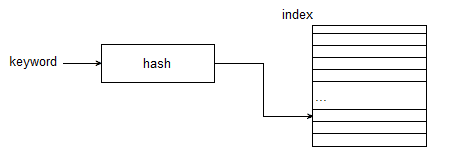
\includegraphics[height=162px, width=472px]{hashtab1.png}
\caption{Хеш табела}
\label{slike:hash1}
\end{figure}

\begin{figure}[here]
\centering
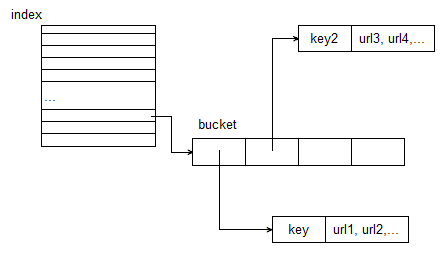
\includegraphics[height=257px, width=446px]{hashtab2.png}
\caption{Смештање елемената у листу хеш табеле}
\label{slike:hash2}
\end{figure}

Дакле, ако постоје \emph{k} кључних речи и \emph{b} листа у хеш табели, потребно је имати одговарајућу процедуру која ће смештати кључну реч у одговарајућу листу. \\

\subsubsection{Дефинисање хеш функције}

Претпоставимо да имамо \emph{b} листи у хеш табели. Хеш функција треба да узме као улазне податке кључну реч и број листи, а да као излаз да вредност између 0 и \emph{b}-1 (слика \ref{slike:hashstring}).

\begin{figure}[here]
\centering
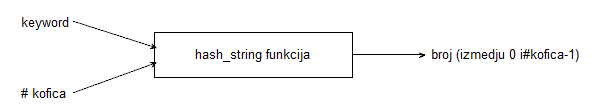
\includegraphics[height=75px, width=400px]{hashstring.png}
\caption{Hash функција}
\label{slike:hashstring}
\end{figure}

Најједноставније решење би било да функција узима прво слово кључне речи, налази \emph{ASCII}\index{ASCII@\emph{ASCII}}\footnote{скраћеница од „Амерички стандардни код за размену података“ (енгл. \emph{American Standard Code for Information Interchange}) је кодни распоред заснован на латиничном писму које се користи у енглеском језику. Сваки карактер добија одговарајући број. На пример. ,,а'' има број 98, ,,А'' 67, ,,б'' 99, итд.} кодни број карактера који је прво слово кључне речи, затим дели тај број по модулу \emph{b} (где је \emph{b} број листи хеш табеле) и резултат тог дељења даје индексни број листе у коју ће кључна реч бити смештена.

\begin{lstlisting}[caption = Лоша хеш функција, label = {lst:badhash}, numbers = left]
def bad_hash_string (keyword, buckets):
    return ord(keyword[0]%buckets)
\end{lstlisting}

Да би се анализирало да ли је ово добар начин да се равномерно поделе кључне речи по листама у табели, потребно је тестирати ову функцију\index{hash!hash funkcija@хеш функција}. Следећа функција ће послужити да би се видела расподела елемената по листама хеш табеле:

\begin{lstlisting}[caption = Тестирање хеш функције, label={lst:hashtest}, numbers=left]
def test_hash_function(func, keys, size):
   results = [0] * size
   keys_used = []
   for w in keys:
       if w not in keys_used:
           hv = func(w, size)
           results[hv] += 1
           keys_used.append(w)
   return results
\end{lstlisting}
%\pagebreak

Ова функција ће узети као улазне податке саму хеш функцију, кључне речи (као листу ниски) и број листи хеш табеле. Резултат који се добија није најбољи:

\begin{lstlisting}[caption = Резултат тестирања лоше hash функције, label={lst:resultstest}]
words = get_page('http://www.gutenberg.org/files/1497/1497.txt').split()
# uzimaju se sve reci iz Platonove ,,Republike''

counts = test_hash_function(bad_hash_string, words, 12)
# rezultat testiranja se smesta u promenljivu counts

print counts
[725, 1509, 1066, 1622, 1764, 834, 1457, 2065, 1398, 750, 1045, 935]
\end{lstlisting}

Као што се види, у једној листи је 725 речи, а у другој преко 2000. То није добро, јер је циљ распоредити речи што уједначеније, а тиме и убрзати процес тражења кључних речи у хеш табели.

Бољи начин прављења хеш функције био би да се зависно од кључне речи, саберу ASCII к\^{о}дови свих знакова у тој речи, затим се тај збир подели по модулу броја листи хеш табеле и резултат дељења ће бити индексни број листе у коју се смешта кључна реч.

\begin{lstlisting}[caption=Боља хеш функција, label={lst:betterhash}, numbers = left]
def hash_string(keyword, buckets):
    h = 0
    for c in keyword:
        h = (h + ord(c))%buckets
    return h
\end{lstlisting}

Ако се тестира нова хеш функција\index{hash!hash funkcija@hash функција} за исте улазне вредности, резултати ће бити нешто бољи:

\begin{lstlisting}[caption = Тестирање боље хеш функције,label={lst:betterhashtest}]
counts = test_hash_function(hash_string, words, 12)
# rezultat testiranja nove funkcije
[1363, 1235, 1252, 1257, 1285, 1256, 1219, 1252, 1290, 1241, 1217, 1303]
\end{lstlisting}

Очигледно је расподела боља, мада свакако није идеална. Најмање попуњена листа има 1217 речи, а највише преко 1360. Тражење идеалне расподеле је предмет шире расправе (погледати \cite[поглавље~6.4]{Knuth1998ACP} \cite[поглавље~3]{cormen2001introduction} или \cite{artofhashing} и сл.), тако да ће за потребе овог рада, бити усвојена ова функција као пример добре расподеле.

%\pagebreak

\subsubsection{Прављење празне хеш табеле}

Ако је познат број листа хеш табеле, потребно је прво направити празну хеш табелу у коју ће се касније смештати подаци. Питање је какву структуру одабрати за ову табелу\index{hash!hash tabela@hash табела}. Следи к\^{о}д који прави празну хеш табелу од \emph{n} листи.

\begin{lstlisting}[caption=Празна хеш табела, label={lst:emptyhash}, numbers = left]
def make_hashtable(n):
    i = 0
    table = []
    while i < n:
        table.append([])
        i = i + 1
    return table
\end{lstlisting}

\subsubsection{Налажење одговарајуће листе}

Ако је потребно сместити податке у листе хеш табеле, онда мора бити познат индексни број листе у коју ће се сместити податак. Такође, кад се укаже потреба за  претраживањем података, опет мора бити познат индексни број листе у којој се налази тражени елемент. Дакле, потребне су две процедуре, нпр. \emph{add} и \emph{lookup}, прва која ће да додаје елементе у хеш табелу, а друга која ће да тражи одговарајући податак у табели. Претпоставимо да већ постоје функције \emph{hash\_string}(видети к\^{о}д \ref{lst:betterhash}) и \emph{make\_hashtable}(видети к\^{о}д \ref{lst:emptyhash}) које су раније наведене.

\begin{lstlisting}[caption= \emph{add} и \emph{lookup} функције, label={lst:addlookup}, numbers = left]
# pomocna funkcija: vraca indeksni broj liste u odnosu na keyword
def hashtable_get_bucket(htable, keyword):
    return htable[hash_string(keyword, len(htable))]


# funkcija dodavanja u tabelu
def hashtable_add(htable, key, value):
    return hashtable_get_bucket(htable, key).append([key, value])


# funkcija trazenja
def hashtable_lookup(htable, key):
    bucket = hashtable_get_bucket(htable, key)
    for i in bucket:
        if i[0]==key:
            return i[1]
    return None
\end{lstlisting}

На почетку наведеног к\^{о}да је дата помоћна функција \emph{hashtable\_get\_bucket} јер се употребљава у обе тражене функције за исту сврху - враћање индексног броја листе за одговарајућу кључну реч.

\subsubsection{Коришћење мапе уместо листе}

Уместо листе за прављење хеш табеле, могуће је користити мапе (погледати под \ref{subsec:maps}). Да би се имплементирала таква структура, потребно је преправити претходно наведене процедуре: \textbf{crawl\_web}, \textbf{add\_to\_index} и \textbf{lookup}, тако да могу да раде са мапама, а не са листама. Предност мапа у односу на листе је прегледност и бржи рад. Тако да би алгоритам могао да буде реализован на следећи начин:

\begin{lstlisting}[caption=Мапа уместо листе, label={lst:dictionary}, numbers=left]
def get_page(url):
    try:
        import urllib
        return urllib.urlopen(url).read()
    except:
        return ""

def union(p,q):
    for e in q:
        if e not in p:
            p.append(e)

def get_next_target(page):
    start_link = page.find('<a href=')
    if start_link == -1:
        return None, 0
    start_quote = page.find('"', start_link)
    end_quote = page.find('"', start_quote + 1)
    url = page[start_quote + 1:end_quote]
    return url, end_quote

def get_all_pages(page):
    while True:
        links = []
        url, endpos = get_next_target(page)
        if url:
            links.append(url)
            page = page[endpos:]
        else:
            break
    return links

# index
def add_to_index(index,keyword,url):
    if keyword in index:
        index[keyword].append(url)
    else:
        index[keyword]=[url]

def add_page_to_index(index,url,content):
    for entry in content.split():
        add_to_index(index, entry, url)

# lookup
def lookup(index, keyword):
    if keyword in index:
        return index[keyword]
    else:
        return None


def crawl_web(seed):
    tocrawl = [seed]
    crawled = []
    index = {} #inicijalizacija mape
    while tocrawl:
        page = tocrawl.pop()
        if page not in crawled:
            content = get_page(page)
            add_page_to_index(index, page, content)
            union(tocrawl, get_all_pages(content))
            crawled.append(page)
    return crawled
\end{lstlisting}

Уколико се упореди брзина рада веб-паука који ради са хеш-табелама са листама и са мапама, долази се до закључка да веб-паук који ради са мапама много брже похрањује податке у хеш табелу. На пример, ако се узме ограничење од 10, 20 или 50 веб страна и упореди рад веб-паука са мапама и листама добијају се  следећи резултати (погледати \ref{sec:dodatakb}):

